%Discuss how development processed, problems encountered and how some features were cut or added.
\chapter{Development Process} %Carsten
Development started the 17th of February and ended the 19th of June, with three week period ranging from 4th to 19th of June. Up until the three period we met once a week, and thereafter met daily. We attempted to distribute work equally, but each of us programmed and wrote about specific parts of the project.

\section{Timeplan} %Cebrail/Jonathan
When we started the project we created a waterfall chart containing our plans for every week. The waterfall chart is a sequential design process. It is designed to get through the project phases and have a product as soon as possible. The phases in our project can be seen in the figure below.
\newline
As we revisited our waterfall model throughout development, our main time plan can be considered to be iterative. The revisits have mainly been to extend features,debugging or optimizing.
\newline
When the waterfall ends and we still have time we will go back and visit the steps and check for new requirements.
\newline
The waterfall gives a good picture of the big phases, but the pre-planned week schedules are not always much help, as they are not dynamic. We can't reconstruct our waterfall every time we meet a conflict. This is here where the timeboxes are handy, which is used to the most detailed part of the time planning - see next subsection. You can check our waterfall timeplan in the appendices, please see Figure~\ref{fig:Waterfall_chart} for that.
\begin{figure}[h]
\centering
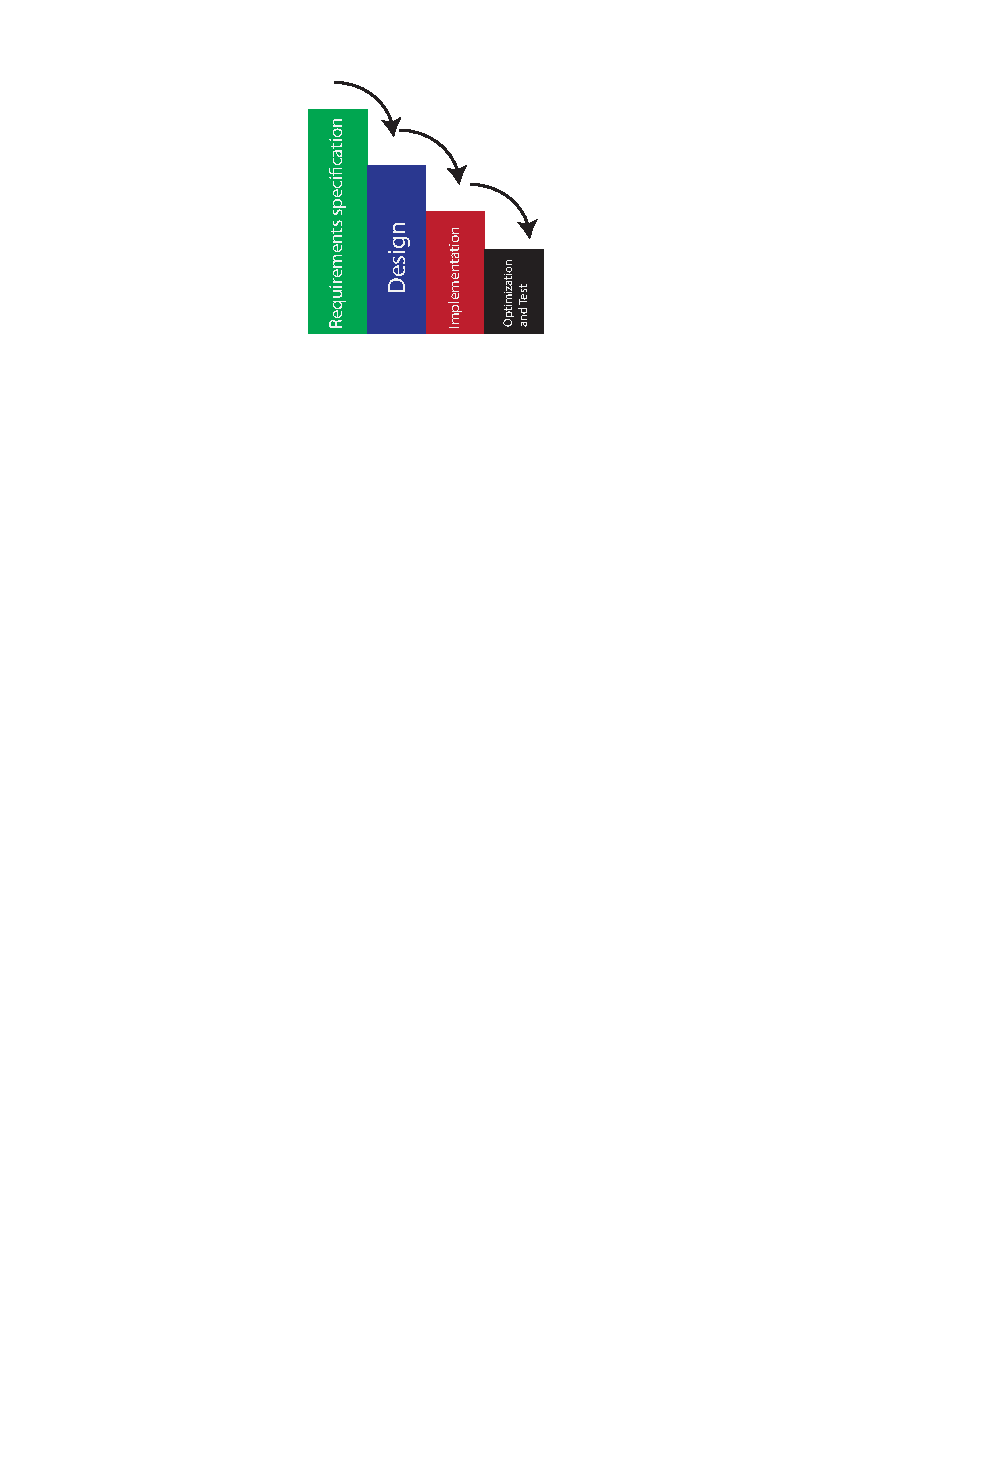
\includegraphics[scale=0.6]{Figures/Waterfall}
\caption{An overview of the waterfall phases.}
\label{fig:Waterfall}
\end{figure}
\newpage

\subsection*{Time Boxing} %Jonathan
We were convinced that using "Time Boxing" would be the way to go. Timeboxing divides The schedule into a number of separate time periods(timeboxes), with each part having its own deliverables, deadline and budget. We used this method to break bigger tasks into smaller tasks with more manageable time frames. What's important is that by the end of each timebox we need are left with a product where if all else fails we can roll back and release our game from an earlier state. The following table shows the timeboxes we have created during the project.
%Please add the following required packages to your document preamble:
%\usepackage[table,xcdraw]{xcolor}
%If you use beamer only pass "xcolor=table" option, i.e. \documentclass[xcolor=table]{beamer}
\begin{table}[h]
\begin{tabular}{llll}
  \rowcolor[HTML]{BBDAFF}
  \textbf{week 8-10}	& \textbf{week 11-13}	& \textbf{week 14-15}	& \textbf{week 16-17}	\\
  Code exercise			& Collision detection	& Level generation		& Graphics				\\
  Class design			& Enemies				& Player				& Level generation		\\
  Game Design			& Input					& 						& Sprites				\\
  \rowcolor[HTML]{BBDAFF} 
  \textbf{week 18}		& \textbf{week 19}		& \textbf{week 20}		& \textbf{week 22}		\\
  Endgame				& Attack				& Animation				& Optimization			\\
  Level generation		& Level generation		& Optimization			& 						\\
  						& Optimization			& Sound					& 						\\
  						& 						& Sprites 				& 						\\
  \rowcolor[HTML]{BBDAFF}
  \textbf{week 23}		& \textbf{week 24}		& \textbf{week 25}		& 						\\
  Attacks				& AI					& Bug Fixes				& 						\\
  Coins					& High score			& Code Polish			& 						\\
  Optimization			& Optimization			& Optimization			& 						\\
\end{tabular}
\caption{The timeplan in timebox format.}
\end{table}

\section{Development Issues} %Cebrail / Jonathan / Carsten
We received the Arduino three weeks after the course started, which was a major setback in implementation. All we could do in this time was design the program structure and time-plans. This skewed our planned agile development. Instead of dynamically designing and implementing additional features, we had to make the most of our time and design for three weeks straight. Usually in agile processes, you make sure to have a working product at the end of each timebox. This was not compatible with our designed framework, since we had taken a lot more features into consideration than possible in a single timebox. It was one very large timebox, more akin to the waterfall process. We could have incrementally implemented the framework after receiving the Arduino, but in the end it would have been slower and more tedious. We had the designs so all we had to do was implement them. In the end we made up for the loss in implementation time by cutting corners in the process and designing a lot ahead.
\newline
Later on, one of the Arduinos burned out. It is not clear what went wrong and it rarely worked. At this time we only had another Leonardo and the Duemilanove. This slowed us down quite a bit as only half of us could program each week. A few weeks later we hit the maximum code size on the Duemilanove, and were left with only a single working Arduino. Development became too slow, until we traded the Duemilanove for another Leonardo.
\newline
General problems with the Arduinos were common. We have also had some issues when uploading code to the Arduino. The screen would be completely black even though the IDE stated the upload was complete. The usual fix was uploading a simple example file from the Arduino library, usually {\tt HelloWorld.ino}. In other cases changing the USB port would solve it. It was probably a sign of incorrect driver installation. Resetting the Arduino during uploading would also sometimes solve it. Other problems were related to the SD card in the Gameduino 2, where we could not upload programs while the SD card was inserted. The SD would get corrupted and a reformatting would be required. Usually this would work, but often only when done through a Mac for unknown reasons.
